% **************************************************************************** %
\chapter{Markante Ereignisse}
\label{chap:markant}
% **************************************************************************** %

Das  Ishikawa-Diagramm   in  Abbildung  \ref{fig:ursache:wirkung}   auf  Seite
\pageref{fig:ursache:wirkung}  stellt  die   drei  wichtigsten  positiven  und
negativen Erfahrungen dar, welche im Verlauf des Projektes gemacht wurden. Die
meisten  dieser   Erfahrungen  wurden   im  Bereich  Projektarbeit   und  Team
Zusammenarbeit gemacht. Die technische Herausforderung  des Projekts 4 war vom
Modul gegeben. Es  wurden erstmals  alle erlernten  Methoden und  Theorien bei
einem Projekt verwendet, wobei die F\"ahigkeiten aller Teammitglieder zu sehen
waren.

Zu  Beginn  des  Projektes  wurden  sehr  schnell  Fortschritte  erzielt,  wie
zum  Beispiel die  Fertigstellung  des ersten  Sensorplatinen-Prototypen. Dies
stimmte das  gesamte Team optimistisch,  dass wir unser  Projektziel erreichen
k\"onnten. Dies war zu  Beginn alles andere als  klar. Die Zusammensetzung aus
drei ETH  Abg\"angern und  drei berufsbegleitend Studierenden,  welche jeweils
nur wenig Projekt- und Elektronikerfahrung  hatten, liess ein sehr schwieriges
Projekt erahnen. Trotz  dieser schwierigen Voraussetzungen war  das ganze Team
sehr motiviert und auch bereit ein hochwertiges Produkt zu entwickeln.

Die beste  positive Erfahrung wurde  bei der Zusammenarbeit  gemacht. Das Team
konnte kaum unterschiedlicher sein. Dies hatte  jedoch keinen Einfluss auf die
Arbeitsmoral  der Mitglieder. Alle  gaben  ihr Bestes  und  jeder konnte  sein
K\"onnen unter  Beweis stellen. Was  unter dem  st\"andigen Stress  im Projekt
keine Selbstverst\"andlichkeit  darstellt. Ebenfalls eine sehr  gute Erfahrung
wurde beim Arbeiten  am Fachbericht gemacht. Der Dokumentationsverantwortliche
hatte  gl\"ucklicherweise   bereits  einige  Erfahrungen  mit   Schreiben  von
Berichten. Dadurch  lief  die  Planung  der  Dokumentation  sehr  planm\"assig
und  ohne  nennenswerte Verz\"ogerungen. Er  konnte  die  einzelnen Teile  gut
zusammenf\"uhren und  ermahnte alle  Teammitglieder regelm\"assig,  ihren Teil
beizutragen.

Es wurden  jedoch auch negative Erfahrungen  gemacht, welche vor allem  in der
zweiten Projekth\"alfte auftraten. Die  Softwareentwicklung wurde planm\"assig
in dieser  Zeit begonnen und  war bereits  nach zwei Wochen  in Verzug. Leider
konnte dieser  Verzug w\"ahrend  mehreren Wochen  nicht behoben  werden, trotz
starker  Bem\"uhungen  vom  halben   Team. Ein  st\"andiges  Problem  war  die
Zuverl\"assigkeit  einiger  Teammitglieder. Es  kam   einige  Male  vor,  dass
zugeteilte Aufgaben nicht wie  erwartet erledigt wurden. Dieses Problem konnte
gl\"ucklicherweise bis zum Projektende behoben werden.

{\begin{a3pages}
    \begin{tikzpicture}[remember picture,overlay]
        \node at (current page.center) {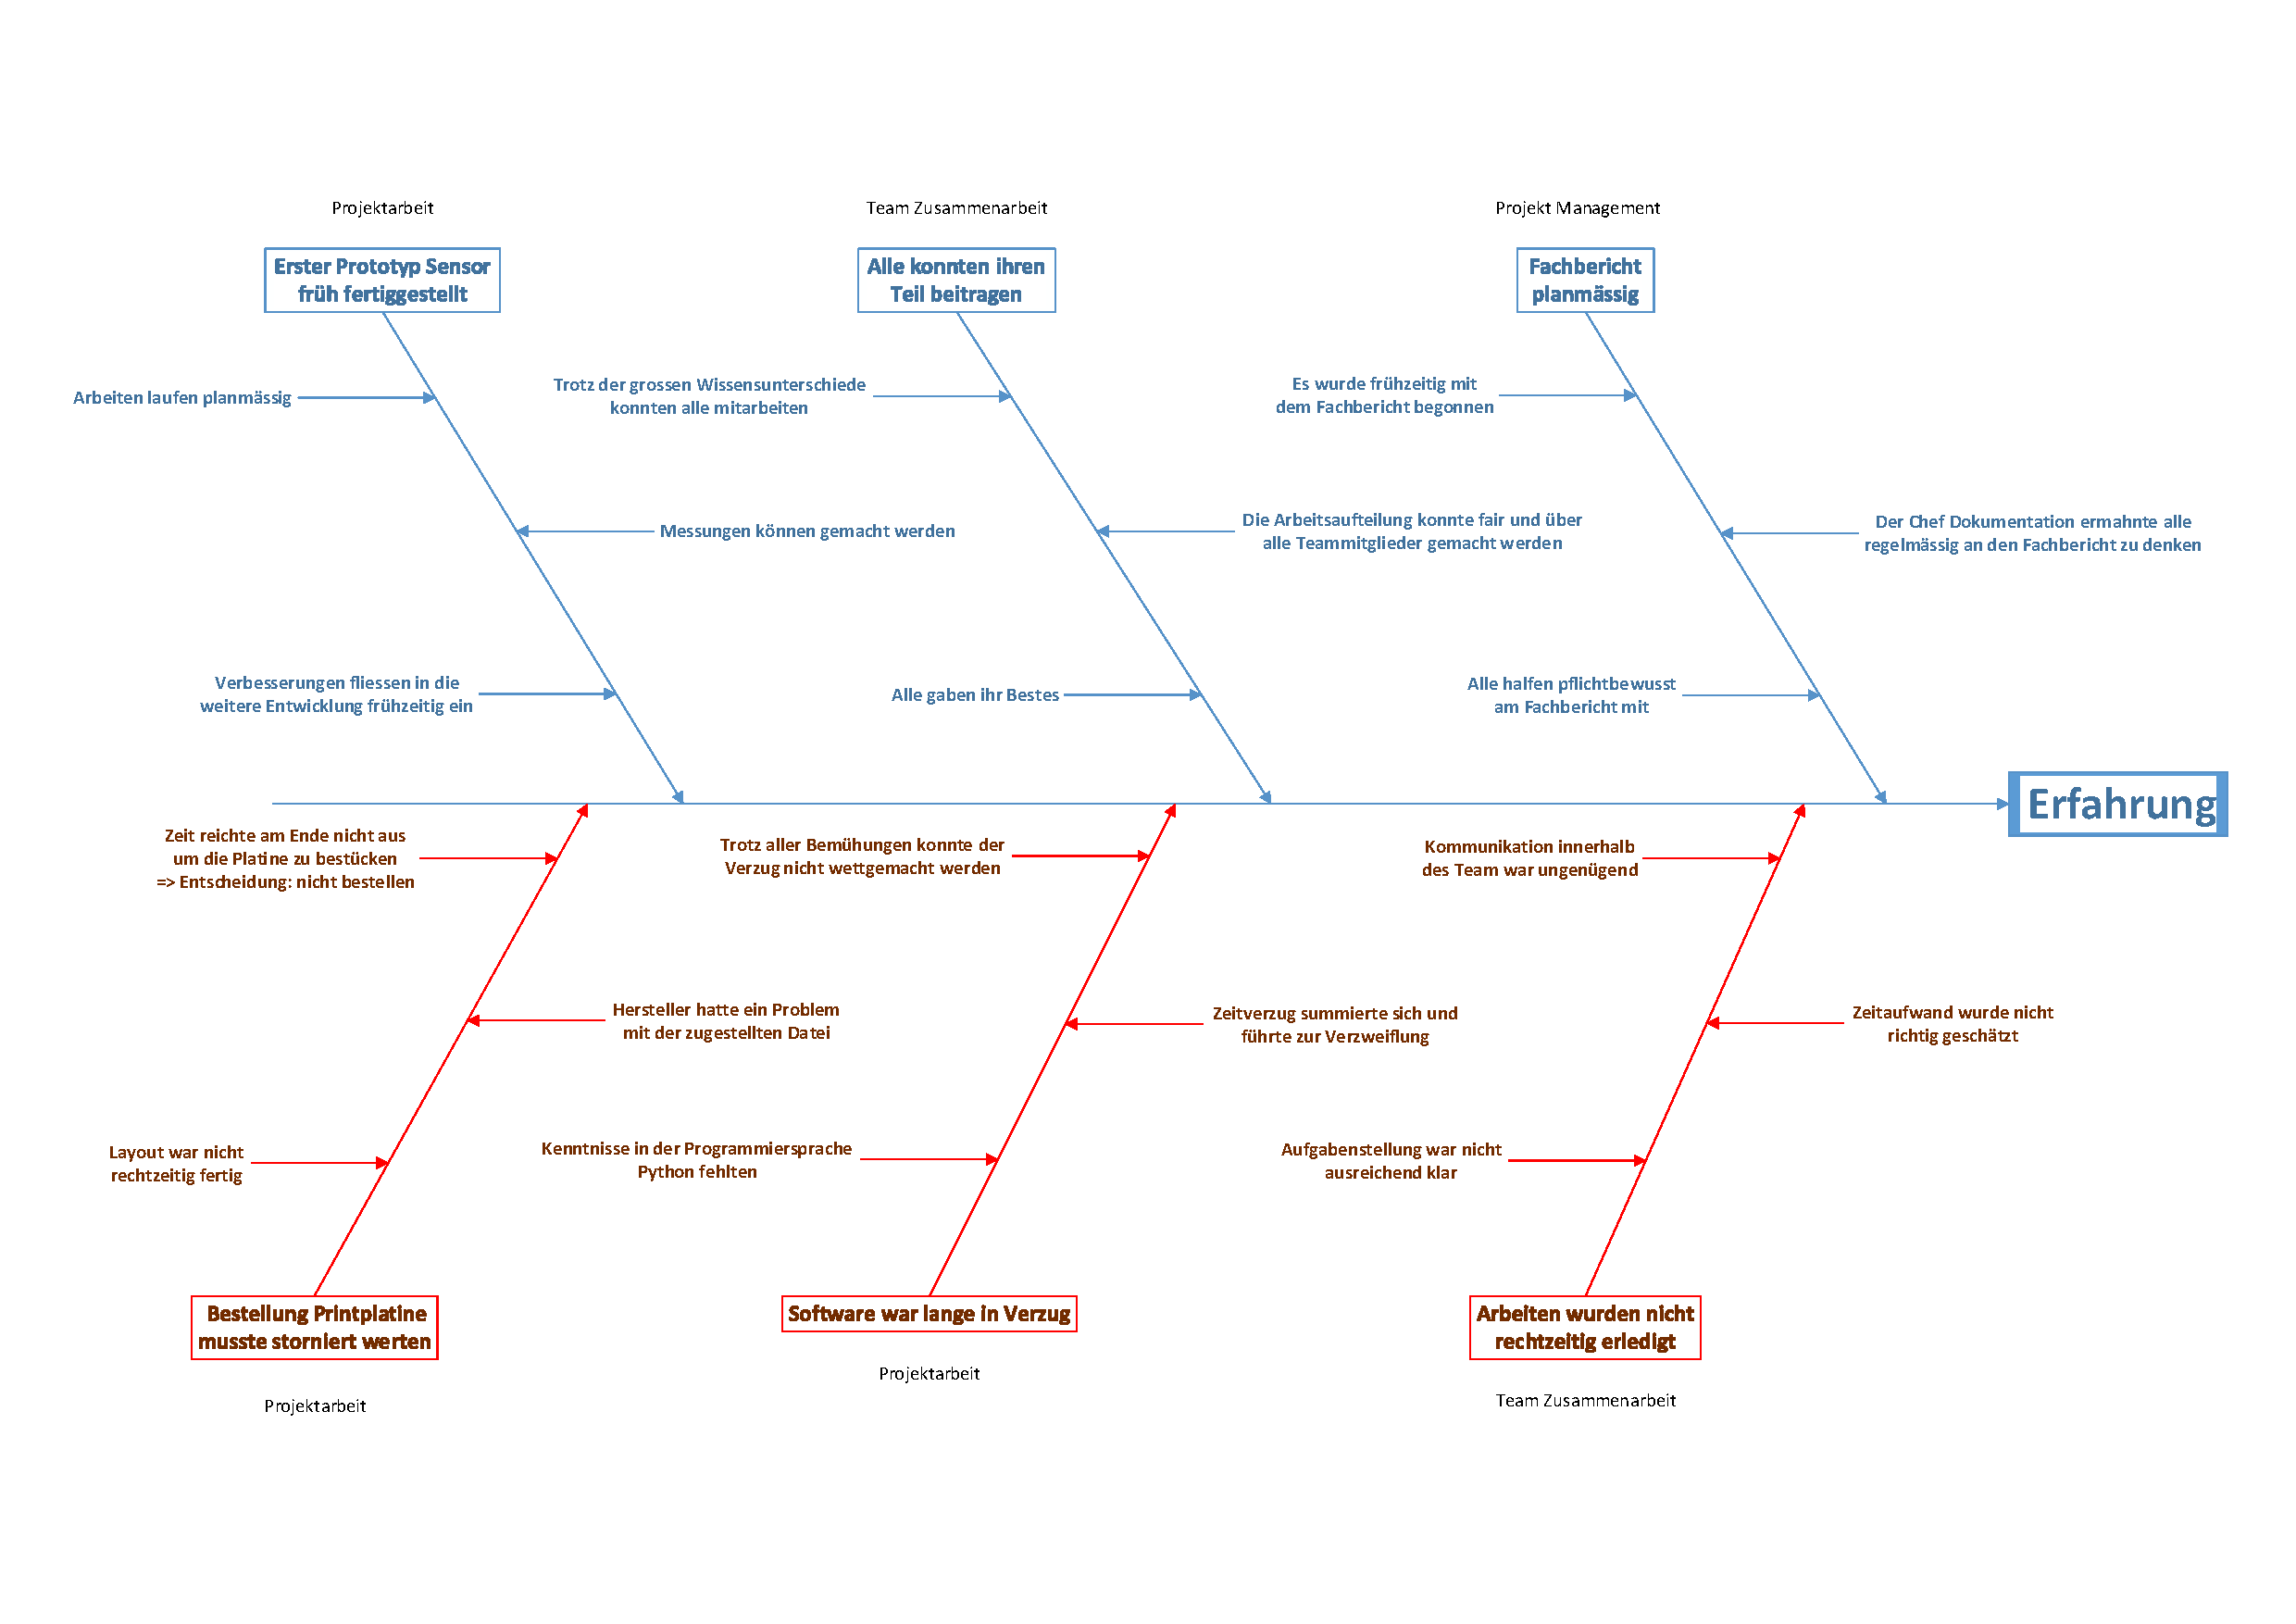
\includegraphics[width=0.85\paperwidth]{images/ursache-wirkung.pdf}};
    \end{tikzpicture}
    \vspace*{202mm}
    \figcaption{Ursache-Wirkung-Diagramm f\"ur unser Projekt}
    \label{fig:ursache:wirkung}
\end{a3pages}}
